%%=============================================================================
%% netadmin-voorbereidingen
%%=============================================================================

\chapter{Netadmin - Voorbereidingen}%
\label{ch:netadmin-voorbereidingen}

Voorafgaand aan de ontwikkeling van de nieuwe website worden verschillende voorbereidingen getroffen om een solide basis te leggen voor het project. Eerst worden er metingen gedaan om na te gaan hoeveel tijd de netwerkbeheerder dagelijks moet investeren om de registraties van die dag te behandelen. Daarna wordt nagegaan wat van de nieuwe website verwacht wordt, hoe die geïmplementeerd kan worden in de huidige infrastructuur, en hoe de ontwikkeling zal aangepakt worden.

\section{Tijdmetingen IP-registraties}
Zoals beschreven in hoofdstuk \ref{ch:voorgeschiedenis}, ontvangen de netwerkbeheerders van UGent dagelijks meerdere e-mails met IP-registraties van gebruikers. Nadat de netwerkbeheerder heeft beoordeeld of de registratie geschikt is voor uitvoering, moet deze inloggen op de server waar de subnetbestanden zich bevinden. Vervolgens verkrijgt de netwerkbeheerder de juiste privileges door over te schakelen naar de gebruiker die wordt gebruikt voor registraties, om vervolgens de benodigde acties uit te voeren om de registratie te voltooien. Als het subnet niet in de e-mail staat, zoekt de netwerkbeheerder eerst het subnet op, voert het commando in, plakt de inhoud van de e-mail in het bestand en slaat het bestand vervolgens op als er geen verdere wijzigingen nodig zijn. Indien het subnet vol is, voert de netwerkbeheerder opruimacties uit.

Na elke registratie wordt de e-mail met de uitgevoerde registratie verplaatst naar een aparte map in de mailbox. Deze map wordt later gebruikt om te achterhalen welke registraties afgehandeld zijn. Niettemin is het niet mogelijk om op basis hiervan te achterhalen wie wanneer welke registratie heeft verwerkt.

\subsection{Tijdmetingen - aanpak}
Om het dagelijkse tijdsverbruik te meten, is besloten om gedurende 13 opeenvolgende werkdagen alle registraties dagelijks te bundelen en deze te laten uitvoeren door de waarnemer. Bij aanvang van de metingen is de waarnemer al ingelogd op de juiste server in de juiste map en onder de gebruiker die daarvoor gebruikt wordt. Elke registratie wordt afzonderlijk gemeten en genoteerd in een excelbestand. Dit excelbestand zal gebruikt worden om te bepalen hoeveel tijd er kan worden bespaard door de registraties te automatiseren. Deze metingen zijn terug te vinden in bijlage 1: metingen\_preimplementatie.xlsx.

\subsection{Tijdmetingen - analyse}
Op basis van de meetresultaten die terug te vinden zijn in figuur \ref{fig:tijdverbruik_metingen}, blijkt dat het aanmaken, wijzigen en verwijderen van registraties een aanzienlijke tijd in beslag neemt voor netwerkbeheerders. Dagelijks wordt er gemiddeld 17 minuten en 54 seconden besteed aan het exlusief uitvoeren van registratietaken, hierbij wordt geen rekening gehouden met variabelen zoals het aantal te verwerken registraties, de tijd die verloren gaat aan het verbinden met de server, het starten van de handmatige registratieprocessen of andere externe factoren. Deze bevindingen benadrukken de noodzaak om het beheer van IP-registraties te verbeteren en te automatiseren, wat een significante tijdsbesparing en efficiëntiewinst kan opleveren voor netwerkbeheerders.

\begin{figure}[H]
    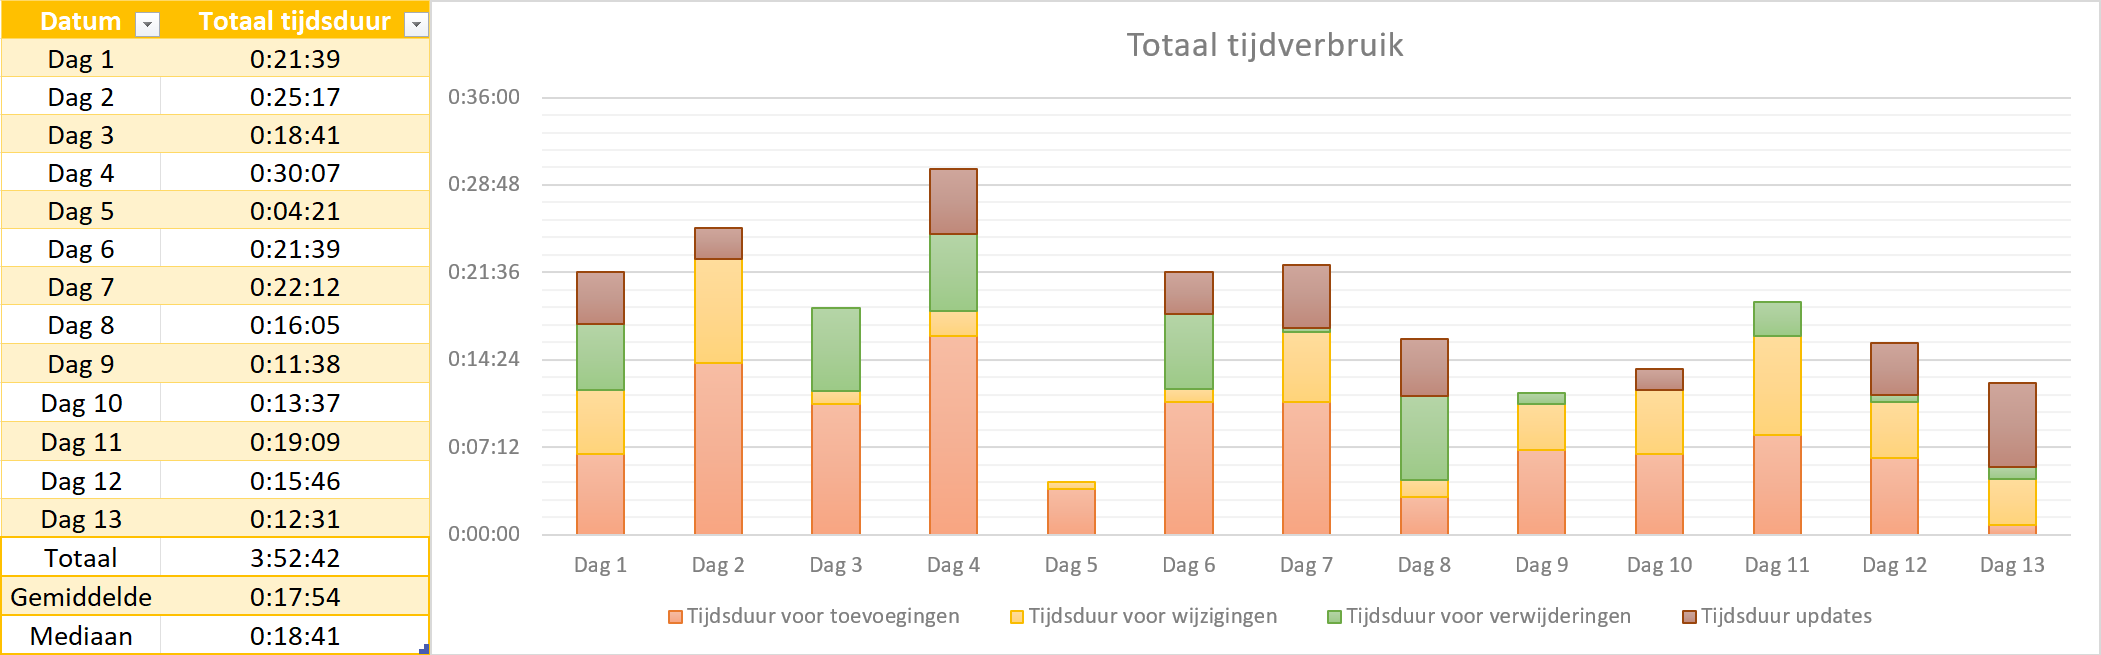
\includegraphics[width=16cm]{grafiek_totaal_tijdverbruik.png}
    \caption{Tabel en grafiek met totaal tijdverbruik tijdens metingen}
    \label{fig:tijdverbruik_metingen}
\end{figure}

\section{Analyse van de oude registratie website}
Voordat het ontwikkelingsproces van start gaat, wordt de bestaande website grondig geëvalueerd om te bepalen welke functionaliteiten kunnen worden overgenomen in de nieuwe website. Dit omvat een diepgaande analyse van de bestaande processen en het identificeren van de vereisten voor de nieuwe website. Flowcharts worden gemaakt om de onderliggende processen te visualiseren en een duidelijk beeld te krijgen van de vereiste functionaliteiten. Deze flowcharts zijn niet definitief en dienen slechts als leidraad om enkele belangrijke stappen weer te geven.

\subsection{Flowcharts van gewenste functionaliteiten}
Er worden vijf flowcharts gemaakt voor acties die mogelijk moeten zijn op de nieuwe website. Deze flowcharts zijn niet bindend en geven slechts een leidraad om op voort te bouwen aan de website.
De eerste functie die elke ingelogde gebruiker op de website zal moeten kunnen, is het opvragen van bestaande registraties. De flowchart hiervoor is terug te vinden in figuur  \ref{fig:flowchart_hostinfo_opvragen}. Eens de gebruiker de juiste registratie gevonden heeft, kan die de registratie desgewenst aanpassen zoals weergegeven in figuur \ref{fig:flowchart_registratie_wijzigen}. Naast het wijzigen en verwijderen van registraties zullen er ook registraties moeten kunnen aangemaakt worden, een mogelijke flow hiervoor is terug te vinden in figuur \ref{fig:flowchart_nieuwe_registratie}.
De netwerkbeheerders zullen een eigen pagina nodig hebben waar ze de nieuwe/gewijzigde registraties kunnen controleren en al dan niet goed- of afkeuren. Een mogelijke methode hiervoor is weergegeven in \ref{fig:flowchart_controle_Wijzigingen}. In sommige gevallen kan het voorkomen dat een subnet vol zit. In dat geval zal de netwerkbeheerder oudere registraties moeten kunnen verwijderen. Deze flowchart is terug te vinden in \ref{fig:flowchart_subnet_opkuisen}. Daarnaast zijn deze vijf flowcharts ook terug te vinden in bijlages twee tot en met zes.

\begin{figure}[H]
	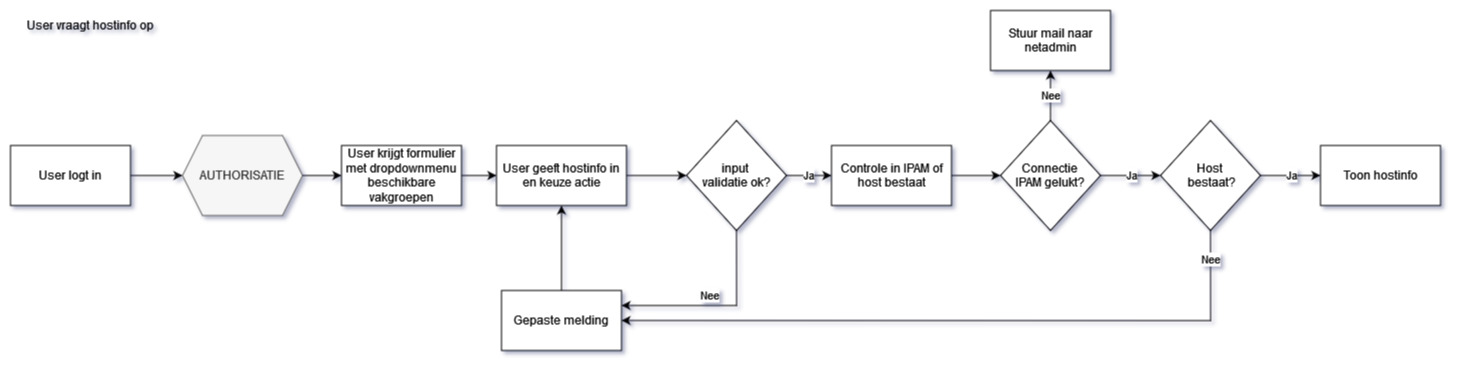
\includegraphics[width=16cm]{Flowchart_Hostinfo opvragen.jpg}
	\caption{Hostinfo opvragen}
	\label{fig:flowchart_hostinfo_opvragen}
\end{figure}
\begin{figure}[H]
    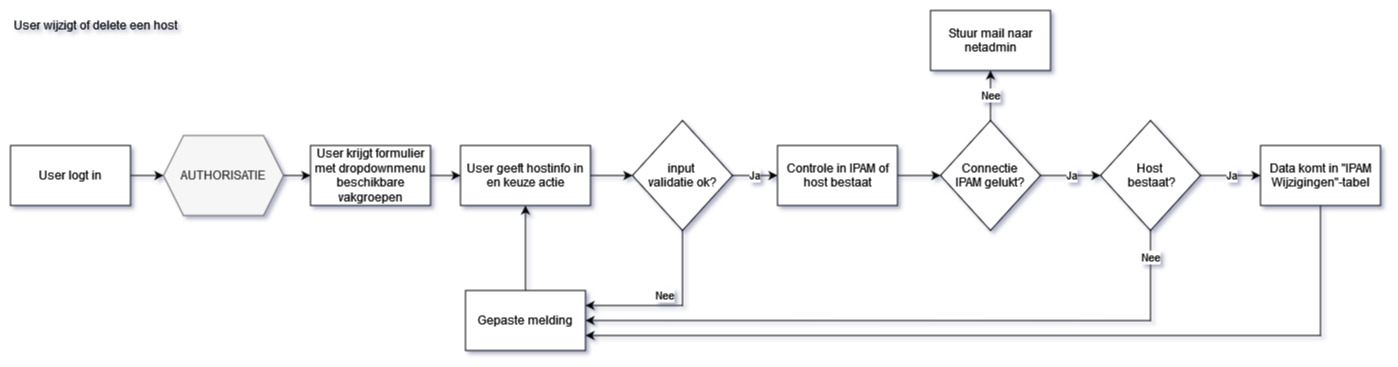
\includegraphics[width=16cm]{Flowchart_Registratie verwijderen of wijzigen.jpg}
    \caption{Registratie wijzigen}
    \label{fig:flowchart_registratie_wijzigen}
\end{figure}
\begin{figure}[H]
    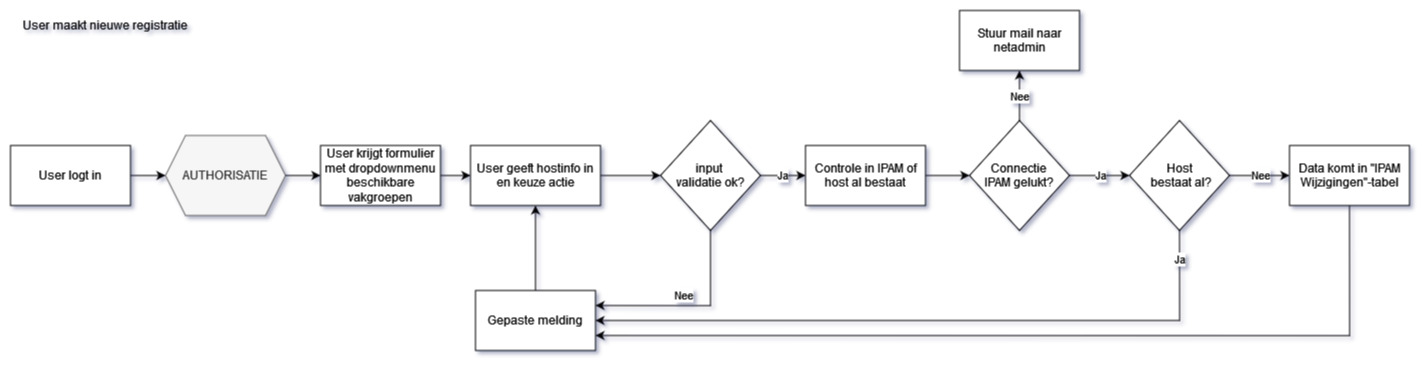
\includegraphics[width=16cm]{Flowchart_Nieuwe registratie.jpg}
    \caption{Nieuwe registratie aanmaken}
    \label{fig:flowchart_nieuwe_registratie}
\end{figure}
\begin{figure}[H]
    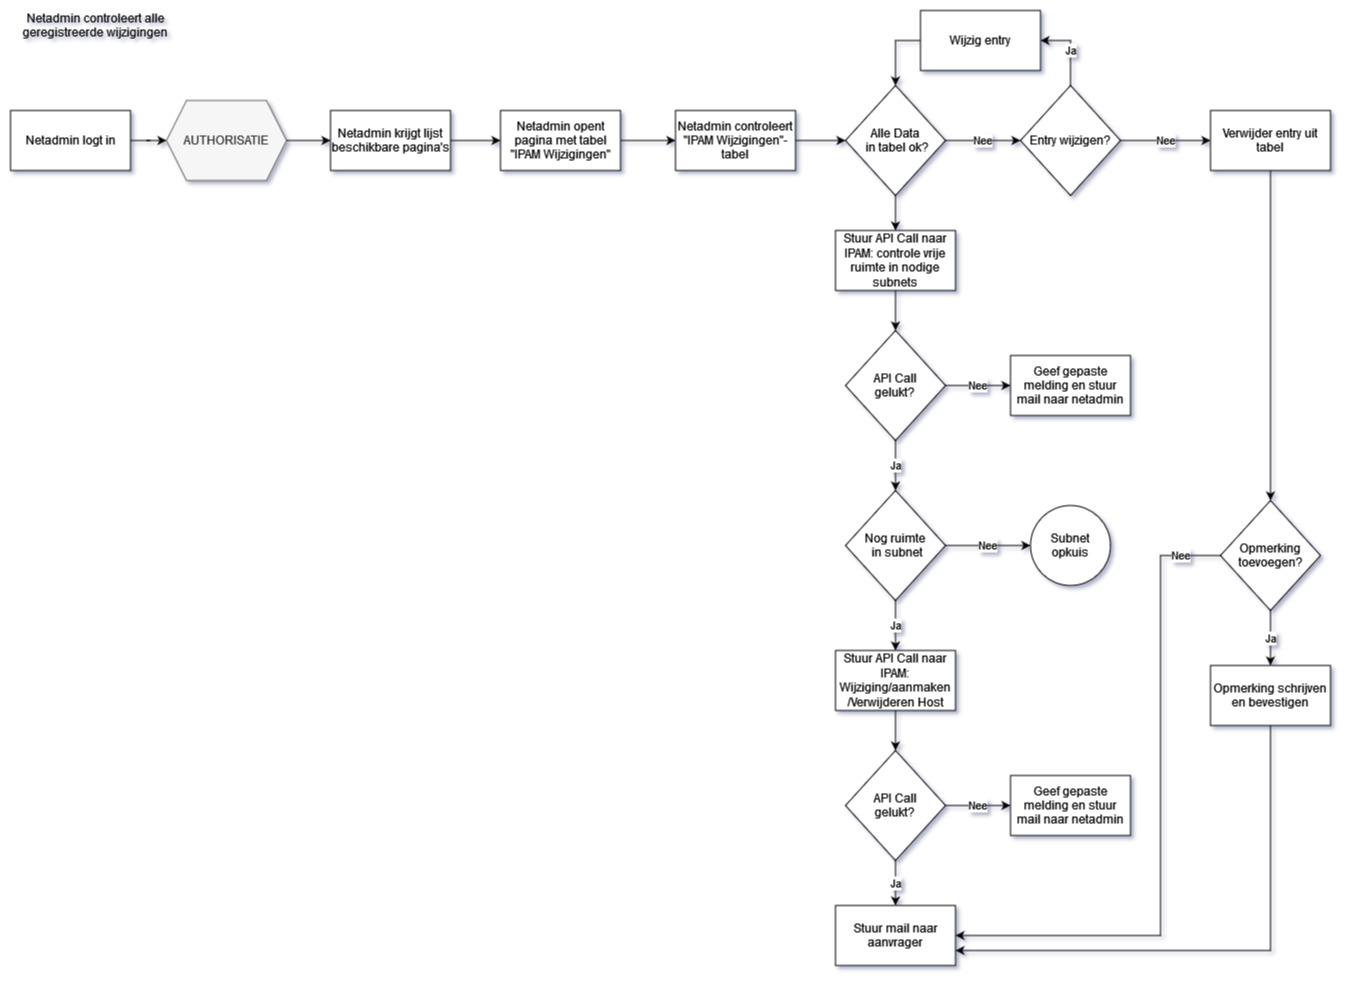
\includegraphics[width=16cm]{Flowchart_Controle IPAM wijzigingen.jpg}
    \caption{Controle wijzigingen}
    \label{fig:flowchart_controle_Wijzigingen}
\end{figure}
\begin{figure}[H]
    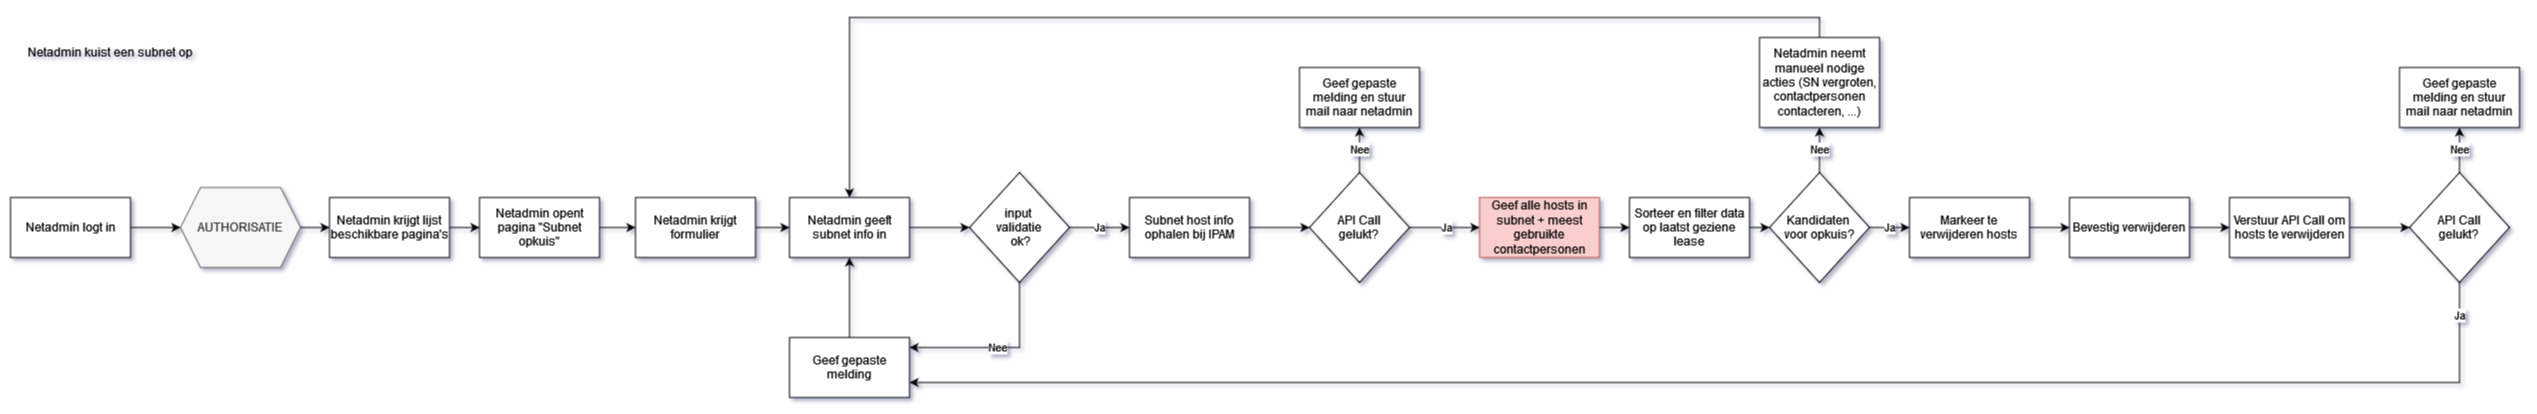
\includegraphics[width=16cm]{Flowchart_Subnet opkuis.jpg}
    \caption{Subnet opschonen}
    \label{fig:flowchart_subnet_opkuisen}
\end{figure}

\section{Integratie binnen de Infrastructuur van UGent}
De integratie van de nieuwe website binnen de infrastructuur van UGent vereist specifieke overwegingen. Eerdere pogingen om de netadmin website te vernieuwen zijn mislukt vanwege de complexiteit van de materie en de verouderde code. Het is essentieel dat de nieuwe website enkele jaren kan meegaan en kan voldoen aan de eisen van UGent. Er wordt besloten om PHP te gebruiken voor de ontwikkeling, gezien de mogelijkheid om Python-scripts aan te roepen, waardoor het project kan worden geïntegreerd in de bestaande infrastructuur.

\section{Agile Ontwikkelinsaanpak}
Zoals eerder vermeld in Sectie \ref{agile}, wordt een Agile aanpak gehanteerd voor de ontwikkeling van de nieuwe registratie-website. De netwerkbeheerders van UGent, als belangrijke stakeholders, worden actief betrokken bij dit proces \autocite{Salameh2014}. Naast de wekelijkse statusvergaderingen met S. Coppens en A. De Keyzer, zoals beschreven in Sectie \ref{agile}, zijn er ook wekelijkse vergaderingen met de netwerkbeheerders. In deze vergaderingen wordt de voortgang besproken en worden beslissingen genomen over de verdere ontwikkeling van de website.

Om flexibel te kunnen reageren op veranderende eisen en prioriteiten, wordt besloten om een Agile ontwikkelingsaanpak te hanteren.
Zoals beschreven door \textcite{Salameh2014} betekent dit dat het ontwikkelproces van de website iteratief en incrementeel verloopt, waarbij wekelijks updates worden uitgebracht die steevast afgetoetst worden bij de stakeholders, zijnde de netwerkbeheerders.
Daarnaast wordt een GitHub-repository opgezet om de broncode te beheren en een development MySQL-database om de ontwikkeling te ondersteunen en informatie persistent te bewaren.
Al deze voorbereidingen vormen de basis voor een gestructureerde en georganiseerde aanpak van de ontwikkeling van de nieuwe website.
